\section{量子力学の法則}
 量子(quantum)とは,とびとびの値を取るという意味である.歴史的に見れば,連続であってほしい量が,なぜか離散的にあらわれて不思議だということから名前が付けられたようだが,歴史的な流れでつけられた名前が本質を表している保証はないと思う.歴史的な流れは排除して,完成された理論として量子力学を理解するのが,見通しがよいと思う.
\subsection{枠組み}
量子力学の基本的な枠組みを列挙する.\footnote{1から4の意味を理解するよい実験としてStern Gerlachの実験がある.}
\begin{enumerate}
    \item 状態は内積の定義された複素線形空間のnon zeroの元である.\label{axiom.1}
    \item 物理量は状態空間の間の線形写像を与える.\label{axiom.2}
    \item 観測される値は,観測する物理量の固有値のいずれかになる.\label{axiom.3}
    \item 状態$\ket{\psi}$に対する物理量$A$の測定により$a_i$という値を観測する確率は,$\abs{\braket{a_i}{\psi}}^2$である.\label{axiom.4}
    \item 系に対する観測以外の操作は(反)unitary変換で指定される.
    \item 系1と系2の状態空間が$\h_1$,$\h_2$のとき,合成系の状態空間は$\h_1\otimes\h_2$である.
\end{enumerate}

以下で,各法則に関する説明を行う.
    \subsubsection*{状態は内積の定義された複素線形空間のnon zeroの元である.}
    

    ある状態があって,それに$\ket{\psi}$と名前を付ける.可能な状態は$\ket{\psi}$,$\ket{\phi}$,$\ldots$とあるとすると,これらをすべて集めた集合$\h\coloneqq\qty{\ket{\psi},\ket{\phi},\ldots}$を状態空間\footnote{(完備な)内積空間をHilbert空間というので,$\h$と書く.ただし,量子力学の状態空間とは微妙な違いがあり,正定値でない内積が出てきたり,そもそも位置の固有状態がHilbert空間の元でないことなどがあるので,Hilbert空間とは言わないようにしている.}と呼ぶ.$\h$には状態の重ね合わせという演算$+$が入っており,任意の$\ket{\psi},\ket{\phi}\in\h, c_1,c_2\in\C\setminus\qty{0}$に対して$\ket{\chi}=c_1\ket{\psi}+c_2\ket{\phi}$も$\h$の元である.これを数学的には$\h$は線形空間であるということで,物理的には重ね合わせの原理\footnote{量子力学は粒子と波の二重性があるといわれることが多いが,粒子は粒子だと思う.粒子がとる物理量に揺らぎがあり,それらの情報に線形性があるというだけな気がする.実際,基礎方程式のSchr\"{o}dinger方程式は波動方程式ではない.i.e.,時間については一階微分である.}という.
    
    また,$\h$の構造としては,更に内積$(\bullet,\bullet):\h\times\h\to\C$が定義\footnote{数学では$(\psi,c\phi)=c^{*}(\psi,\phi)$と後ろを共役線形に定義するが,物理では$(c\psi,\phi)=c^{*}(\psi,\phi)$と前を共役線形にすることが多い.本稿では後者の定義を用いる.}されており,これを$\braket{\psi}{\phi}\coloneqq(\ket{\psi},\ket{\phi})$と書く.\footnote{ここで,$\bra{\psi}$は$\ket{\psi}$の双対ベクトルである.このように書けるのは,Rieszの表現定理により,$f(\ket{\phi})\in\C$なる線形汎関数$f$と,$(\ket{\psi},\ket{\phi})$なる$\ket{\psi}\in\h$の間にone-to-oneの関係があることが保証されるからである.}
    
    \subsubsection*{物理量は状態空間の間の線形写像を与える.}
    
    位置や運動量などの物理量の観測は(可観測量,Observable)は線形写像$A\colon\h\to\h,\ \ket{\psi}\ \mapsto A\ket{\psi}$を与える.これは物理では演算子,数学では作用素という.特にself adjointのクラスに属するものが,物理量に対応する.
    \subsubsection*{観測される値は,観測する物理量の固有値のいずれかになる.}
    物理量$A$に対し,$A\ket{a_i}=a_i\ket{a_i}$なる関係を持たす$\ket{a_i}\in\h$と$a_i\in\C$があり,それぞれ固有状態(eigenstate),固有値(eigenvalue)という.線形写像がself adjointならば,eigenstateにより完全系を構成することが出来る.i.e., 任意の状態がeigenstateにより
    \begin{align}
        \ket{\psi}=\sum_{i}c_i\ket{a_i}\quad;\quad c_i\in\C
    \end{align}
    なる分解ができる.状態$\ket{\psi}\in\h$に対し,物理量$A$を測定したときに,得られる値は$a_i$のいずれかとなる.これが観測量が離散的になりうる理由である.
    \subsubsection*{状態$\ket{\psi}$に対する物理量$A$の測定により$a_i$という値を観測する確率は,$\abs{\braket{a_i}{\psi}}^2$である.}
    
    観測値は物理量の固有値のどれかを取るが,どれを取るかのルールがある.状態$\ket{\psi}=\sum c_i\ket{a_i}$の状態で,物理量$A$を測定すると, 確率$\abs{\braket{a_i}{\psi}}^2=\abs{c_i}^2$で固有値$a_i$を得る.また,測定後の状態は$\ket{a_i}$になる.
    \subsubsection{系に対する観測以外の操作は(反)unitary変換で指定される.}
    
    系に対する時間発展,回転,平行移動などの操作はunitary変換が指定する.ただし,時間反転は反unitary変換である.Heimitian operator $A$があって,$\exp(iA)$はunitary変換である.すなわち,物理量に対応した系の操作があるということで,これが古典力学で保存量が微小変換の生成子になっていることと対応していることをのちに見る.
    \subsubsection*{系1と系2の状態空間が$\h_1$,$\h_2$のとき,合成系の状態空間は$\h_1\otimes\h_2$である.}
    
    $\h_1=\mathrm{Span}\qty{\ket{a_i}},\ \h_2=\mathrm{Span}\qty{\ket{b_j}}$としたとき,合成系の状態空間は$\h_1\otimes\h_2$である.合成系の基底は$\ket{a_i}\otimes\ket{b_j}$たちである.

\section{内積記法とbra-ket notationについて}
このSectionでは,内積記法とbra-ket notationは同じようで強調点が少し違う\footnote{このtopicの元ネタは\url{http://kir018304.kir.jp/nc/htdocs/?action=common_download_main&upload_id=99}にあるpdf.}ということについて述べる.

\subsection{内積による定義}
\begin{defn}[内積]
 $\h$を線形空間とする.任意の$\psi,\phi\in\h$に対して,演算$\langle\bullet,\bullet\rangle\colon\h\times\h\to\C$が定まり\footnote{$\langle\text{hoge},\text{hoge}\rangle$は不等号$<\text{hoge},\text{hoge}>$ではなくlangle,rangleで挟みましょう.},次を満たすもの\footnote{数学と物理では若干流儀が違って,数学では前の後ろのスロットに対して反線形に定義するのがスタンダードだと思う.また$*$は複素共役のこと.数学で複素共役は$\bar{ }$を使うことが多いと思う.}を内積という.

$\psi,\psi_1,\psi_2,\phi,\phi_1,\phi_2\in\h,\ c\in\C$に対して


\begin{align}
    \langle\phi,\psi_1+\psi_2\rangle&=\langle\phi,\psi_1\rangle+\langle\phi,\psi_2\rangle\\
    \langle\phi_1+\phi_2,\psi\rangle&=\langle\phi_1,\psi\rangle+\langle\phi_2,\psi\rangle\\
     \langle\phi,c\psi\rangle&=c\langle\phi,\psi\rangle\\
    \langle c\phi,\psi\rangle&=c^{*}\langle\phi,\psi\rangle\\
    \langle\phi,\psi\rangle&=\langle\psi,\phi\rangle^{*}
\end{align}
が成り立つ.

内積の定まった線形空間を内積空間という.
\end{defn}

 数学的には量子力学はHilbert空間上(完備な内積空間)で作用素を考えるなどであるので,内積で与えるのが自然らしい.
 
\begin{defn}[内積流のHermitian conjugate]
 任意の(Hermitianでなくてもよい)演算子$A$に対し,$\langle B\phi,\psi\rangle=\langle\phi,A\psi\rangle$なる演算子$B$を$A$のHermitian conjugateといい,$A^{\dagger}\coloneqq B$と定める.
\end{defn}

\subsection{bra-ketによる定義}
内積記法は同じ集合$\h$から取った二つの元に注目するが,bra-ket notationは$\h$とそのdualに対し注目する.
\begin{defn}[bra-ket流のHermitian conjugate]

 写像$\dagger$を
\begin{center}
    \begin{tikzpicture}
    \node (dagger)at(-0.3,0){$\dagger\colon$};
    \node (h)at(0,0){$\h$};
    \node (hstar)at(2,0){$\h^{*}$};
    \node (ket)at(0,-1){$\ket{\psi}$};
    \node (bra)at(2,-1){$\bra{\psi}$};
    
    \node (in1)at(0,-0.5){\rotatebox{90}{$\in$}};
    \node (in2)at(2,-0.5){\rotatebox{90}{$\in$}};
    
    \draw[->](h)--(hstar);
    \draw[|->](ket)--(bra);
    \end{tikzpicture}
\end{center}
で定義する.
\end{defn}

\subsubsection*{お絵かきタイム}
図式で書くと,
\begin{center}
    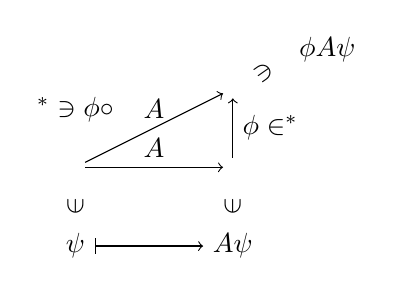
\begin{tikzpicture}
    \node (h1)at(0,0){$\h$};
    \node (h2)at(2,0){$\h$};
    \node (c)at(2,1){$\C$};
    \node (phi)at(0,-1){$\ket{\psi}$};
    \node (Apsi)at(2,-1){$A\ket{\psi}$};
    \node (pAp)at(3.2,1.5){$\bra{\phi}A\ket{\psi}$};
    
    \node (in1)at(0,-0.5){\rotatebox{90}{$\in$}};
    \node (in2)at(2,-0.5){\rotatebox{90}{$\in$}};
    \node (ni)at(2.4,1.2){\rotatebox{215}{$\in$}};
    \node (hstar)at(0,0.73){$\h^{*}\ni\bra{\phi}\circ$};
    
    \draw[->](h1)--node[above]{$A$}(h2);
    \draw[|->](phi)--(Apsi);
    \draw[->](h2)--node[right]{$\bra{\phi}\in\h^{*}$}(c);
    \draw[->](h1)--node[above]{$A$}(c);
    \end{tikzpicture}
\end{center}
のようになる.双対のほうに注目すると
\begin{center}
    \begin{tikzpicture}
    \node (star1) at (0,0){$\h^{*}$};
    \node (star2) at (2,0){$\h^{*}$};
    \node (phi1) at (0,-1){$\bra{\phi}\overset{\leftarrow}{A}$};
    \node (phi2) at (2,-1){$\bra{\phi}$};
    
    \node (in1)at(0,-0.5){\rotatebox{90}{$\in$}};
    \node (in2)at(2,-0.5){\rotatebox{90}{$\in$}};
    
    \draw[<-] (star1)--node[above]{$\overset{\leftarrow}{A}$}(star2);
    \draw[<-|](phi1)--(phi2);
    \end{tikzpicture}
\end{center}
のようになる.$\overset{\leftarrow}{A}$は$A$が$\bra{\phi}$に右からかかっているということを強調する意味である.

すなわち,$\bra{\phi}A\ket{\psi}$は$A$がHermitianかどうかにかかわらず,誤解なしにこのように書け,演算子$A$が左右どちらにかかっているとみてもよい.

誤解を招きやすいがよく用いられる記法として$\braket{\phi}{A\psi}$という記法がある\footnote{Konishi Paffutiの本もこの記法が用いられている.有名な和書では岩波の現代物理学の基礎で用いられており,誤解されていることがネタpdfで言及されている.}.これはbra-ketに似せているが,双対構造が反映されない内積記法である\footnote{ので,私は折衷記法は使わない方がよいと思う.}.これらの記法間の関係は
\begin{align}
    \bra{\phi}A\ket{\psi}=\qty(\ket{\phi})^{\dagger}A\ket{\psi}&=\braket{\phi}{A\psi}=\langle\phi,A\psi\rangle\\
    &=\braket{A^{\dagger}\phi}{\psi}=\langle A^{\dagger}\psi,\psi\rangle\\
    &=\qty(A^{\dagger}\ket{\phi})^{\dagger}\ket{\psi}
\end{align}
である.